\documentclass[a4j,12pt,]{jarticle}
 \usepackage{float}
 \usepackage{siunitx} %%SI単位系用
 \usepackage{amssymb, amsmath}
 \usepackage{ascmac,here,txfonts}
 \usepackage{hyperref}
 \usepackage{listings}
 \usepackage{pxjahyper}
 \usepackage[dvipdfmx]{graphicx}
 \usepackage{amssymb, amsmath}
  \usepackage{listings}
  \usepackage[dvipdfmx]{color}

  \lstset{
    language={Python},
    basicstyle={\ttfamily},
    identifierstyle={\small},
    commentstyle={\small\itshape},
    keywordstyle={\small\bfseries},
    ndkeywordstyle={\small},
    stringstyle={\small\ttfamily},
    frame={single},
    breaklines=true,
    columns=[l]{fullflexible},
    numbers=left,
    xrightmargin=0zw,
    xleftmargin=3zw,
    numberstyle={\scriptsize},
    stepnumber=1,
    numbersep=1zw,
    lineskip=-0.5ex,
  }

\begin{document}

{\noindent\small 第20回報告書 \hfill\today}
\begin{center}
  {\Large 異なるバージョンの Elasticsearch ノードのクラスタリング}
\end{center}
\begin{flushright}
  祖父江匠真 \\
\end{flushright}

\section{概要}
リサイクル館の太陽光パネルの計測データを保存しているElasticsearchシステム(133.71.201.197)はバージョン7.17.6であり, CO\textsubscript{2}データを保存しているElasticsearchシステム(133.71.106.141, 133.71.106.170, 133.71.106.136)はバージョン7.17.9である.

そこで今回は, Docker Compose を使用して, 異なるバージョンである7.17.6 と 7.17.9 の Elasticsearch ノードをクラスタリングすることが可能かどうかを確認するために実施した検証結果について報告する.

\section{Dockerとは}
Dockerは, 軽量で独立したコンテナ型仮想環境用のプラットフォームである.

従来の仮想化では, VMWareなどの仮想化ソフトウェアを用いて, ホストOS上にゲストOSを構築する形式だった.
しかし, DockerはホストOS上にゲストOSなしで独立したコンテナ型の仮想環境として構築される.
Dockerコンテナを利用する場合は, Docker Engineをインストールすることでコンテナの立ち上げ, 停止, 削除といった操作を行うことができる.

\begin{figure}[H]
  \begin{center}
    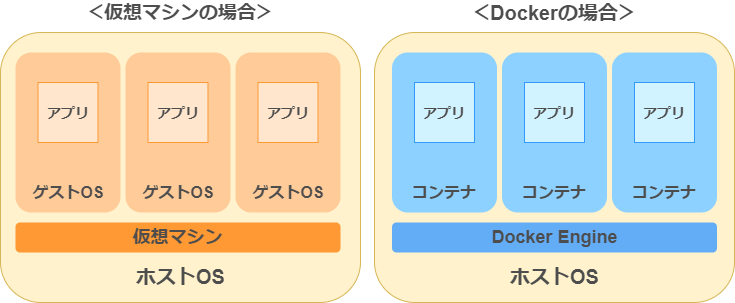
\includegraphics[width=160mm]{docker-vmware.png}
    \caption{仮想マシンとDockerの違い \cite{2}}
    \label{p0}
  \end{center}
\end{figure}

\subsection{コンテナとは}

コンテナは, アプリケーションとそのすべての依存関係(ライブラリ, 実行環境など)をカプセル化した軽量な実行単位である.
Dockerの場合, コンテナの作成にはDockerイメージが必要となる.

\subsection{Dockerイメージとは}

Dockerイメージとは, Dockerコンテナを作成するためのテンプレートであり, Dockerイメージの中には, Docker コンテナの実行に必要な Linux ファイルシステムとメタ情報を含む.

Linux ファイルシステムというのは,  / ディレクトリ以下の /etc /bin /sbin /usr などのディレクトリ階層およびファイルである. 

Docker では, コンテナとして動かしたいアプリケーションが必要とする, 最小限のファイルを Docker イメージの中に入れる. 

さらに, そのアプリケーションを動かすために必要なデフォルトのコマンドや引数の指定, 外に公開するポート番号の情報などの情報がある. これらをメタ情報として, 同じく Docker イメージの中に入れられる 

DockerイメージはDocker Hubやその他のレジストリで共有されており, これらのサービスから取得することが可能である.

今回はElasticsearchの開発元であるElastic社が提供しているElasticsearchのDockerイメージを使って検証を行う.

\begin{figure}[H]
  \begin{center}
    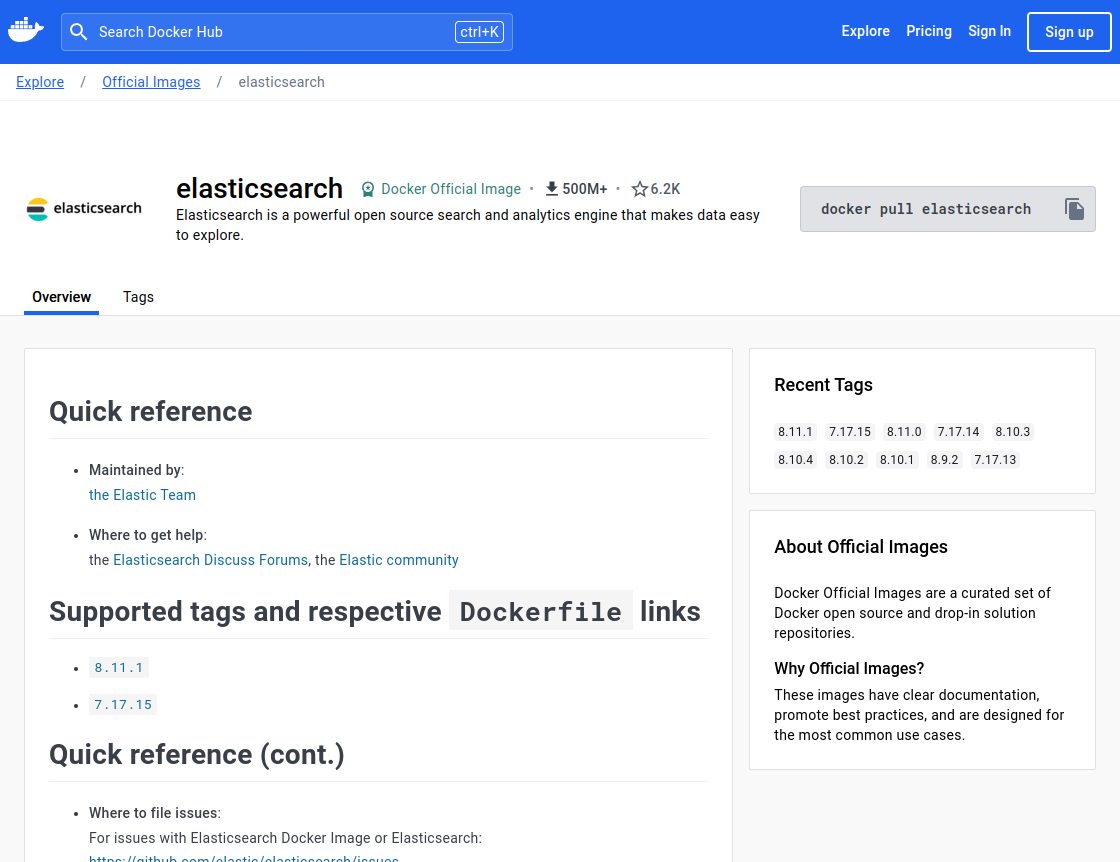
\includegraphics[width=160mm]{elasticsearch-image.png}
    \caption{ElasticsearchのDockerイメージ}
    \label{s0}
  \end{center}
\end{figure}

\section{Docker Composeとは}
Docker Composeは, 複数のコンテナを定義し, 実行するためのツールである. これはYAMLファイルを使用して設定され, 複数のコンテナで協調して動作するアプリケーションの開発を単純化する.

\section{検証環境のセットアップ}
\subsection{全て同じバージョンのElasticsearchを使用したクラスタ構成 (全ノード バージョン 7.17.9)}

Listing \ref{sc1}にクラスタを構成するのに使用したdocker-compose.ymlファイルの内容を記載する.

\begin{lstlisting}[caption=全て同じバージョンのElasticsearchを使用したクラスタを構成するdocker-compose.yml, label=sc1]
version: '2.2'
services:
  es01:
    image: docker.elastic.co/elasticsearch/elasticsearch:7.17.9
    container_name: es01
    environment:
      - node.name=es01
      - cluster.name=es-docker-cluster
      - discovery.seed_hosts=es02,es03
      - cluster.initial_master_nodes=es01,es02,es03
    ports:
      - 9200:9200
    networks:
      - elastic
  es02:
    image: docker.elastic.co/elasticsearch/elasticsearch:7.17.9
    container_name: es02
    environment:
      - node.name=es02
      - cluster.name=es-docker-cluster
      - discovery.seed_hosts=es01,es03
      - cluster.initial_master_nodes=es01,es02,es03
    networks:
      - elastic
  es03:
    image: docker.elastic.co/elasticsearch/elasticsearch:7.17.9
    container_name: es03
    environment:
      - node.name=es03
      - cluster.name=es-docker-cluster
      - discovery.seed_hosts=es01,es02
      - cluster.initial_master_nodes=es01,es02,es03
    networks:
      - elastic

networks:
  elastic:
    driver: bridge
\end{lstlisting}

Listing \ref{sc1}のdocker-compose.ymlファイルで記述している内容について説明する.

\subsubsection*{サービスの定義}
\begin{itemize}
  \item \textbf{es01, es02, es03}: これらはElasticsearchのノード(サーバー)である. 各ノードは異なるコンテナとして定義されている. es01, es02, es03はそれぞれ異なるコンテナ名で, Elasticsearchの異なるインスタンスを実行する.
\end{itemize}

\subsubsection*{各ノードの設定}
\begin{itemize}
  \item \textbf{image}: 使用するDockerイメージ. ここではElasticsearchの7.17.9バージョンを使用している.
  \item \textbf{container\_name}: コンテナに割り当てられる名前.
  \item \textbf{environment}: 環境変数の設定. Elasticsearchのクラスタ設定を含む.
  \item \textbf{ports}: ホストマシンとコンテナ間のポートマッピング. 例えば, `9200:9200`はホストマシンの9200ポートをコンテナの9200ポートにマッピングする.
  \item \textbf{networks}: コンテナ間通信のためのネットワーク設定. ここではelasticネットワークが使用されている.
\end{itemize}

\subsubsection*{ボリュームとネットワークの設定}
\begin{itemize}
  \item \textbf{networks}: デフォルトのドライバであるbridgeドライバを使用するelasticネットワークを定義している. これにより, 異なるコンテナが相互に通信できるようになる.
\end{itemize}

この設定により, Elasticsearchの3ノードを含むクラスタがDocker上で動作するようセットアップされる.

クラスタの起動には, docker compose up -dコマンドを使用する.

docker compose up -dコマンドを実行した後, curlコマンドを使用してクラスタに参加しているノードを一覧表示した結果を図 \ref{p1}に示す.

\begin{figure}[H]
  \begin{center}
    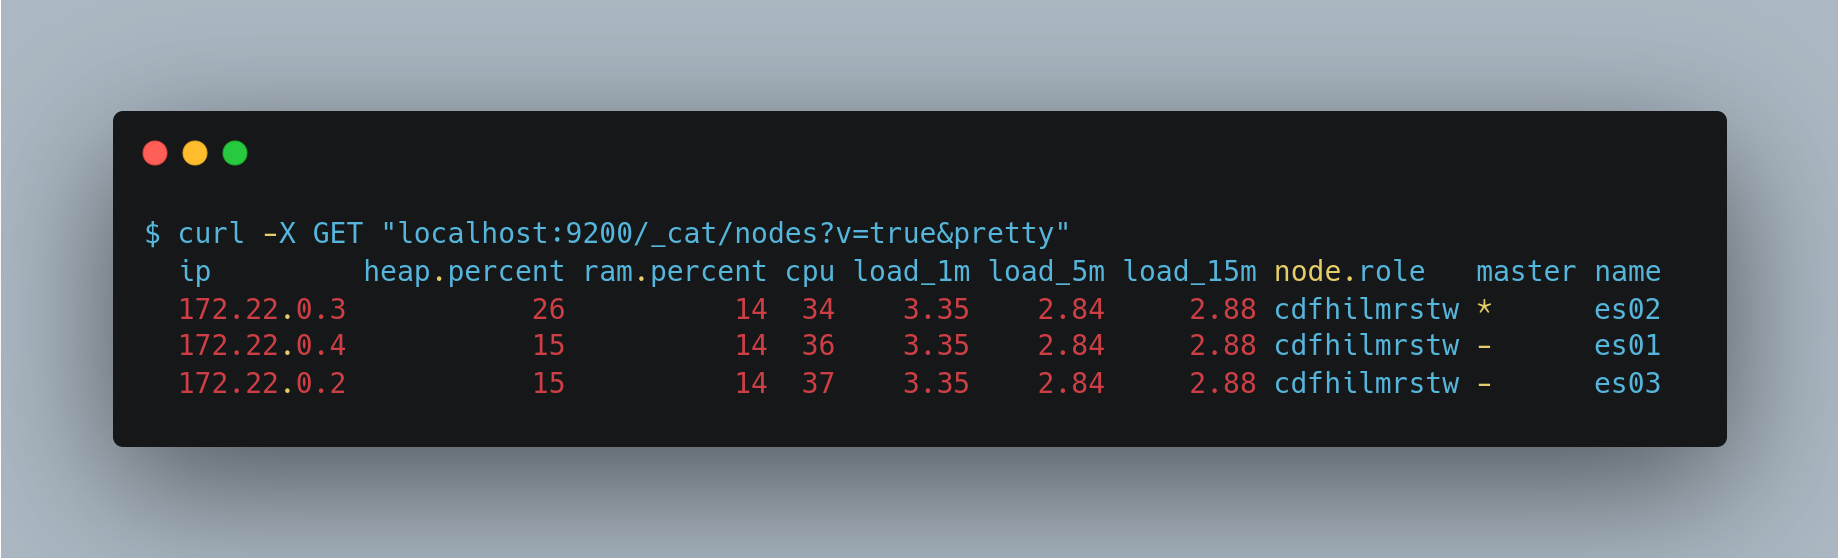
\includegraphics[width=160mm]{curl-same.png}
    \caption{クラスタに参加しているノードを一覧表示した結果}
    \label{p1}
  \end{center}
\end{figure}

図 \ref{p1}より, 3つのノード(es01, es02, es03)すべてが正常にクラスタに参加できていることが確認できる.

\subsection{異なるバージョンのElasticsearchを使用したクラスタ構成 (2ノード バージョン 7.17.9, 1ノード バージョン 7.17.6)}

Listing \ref{sc1}のdocker-compose.ymlのes03のコンテナが使用するDockerイメージをListing \ref{sc2}に変更することで, es03のノードで使用するElasticsearchのバージョンを7.17.9から7.17.6に変更する.

\begin{lstlisting}[caption=Listing \ref{sc1}のdocker-compose.ymlから変更を加えた箇所, label=sc2]
version: '2.2'
services:
  ...
  es03:
    image: docker.elastic.co/elasticsearch/elasticsearch:7.17.6
    ...

...
\end{lstlisting}

変更後, docker compose up -dコマンドを実行してクラスタを起動する.

クラスタの起動後, curlコマンドを使用してクラスタに参加しているノードを一覧表示した結果を図 \ref{p2}に示す.

\begin{figure}[H]
  \begin{center}
    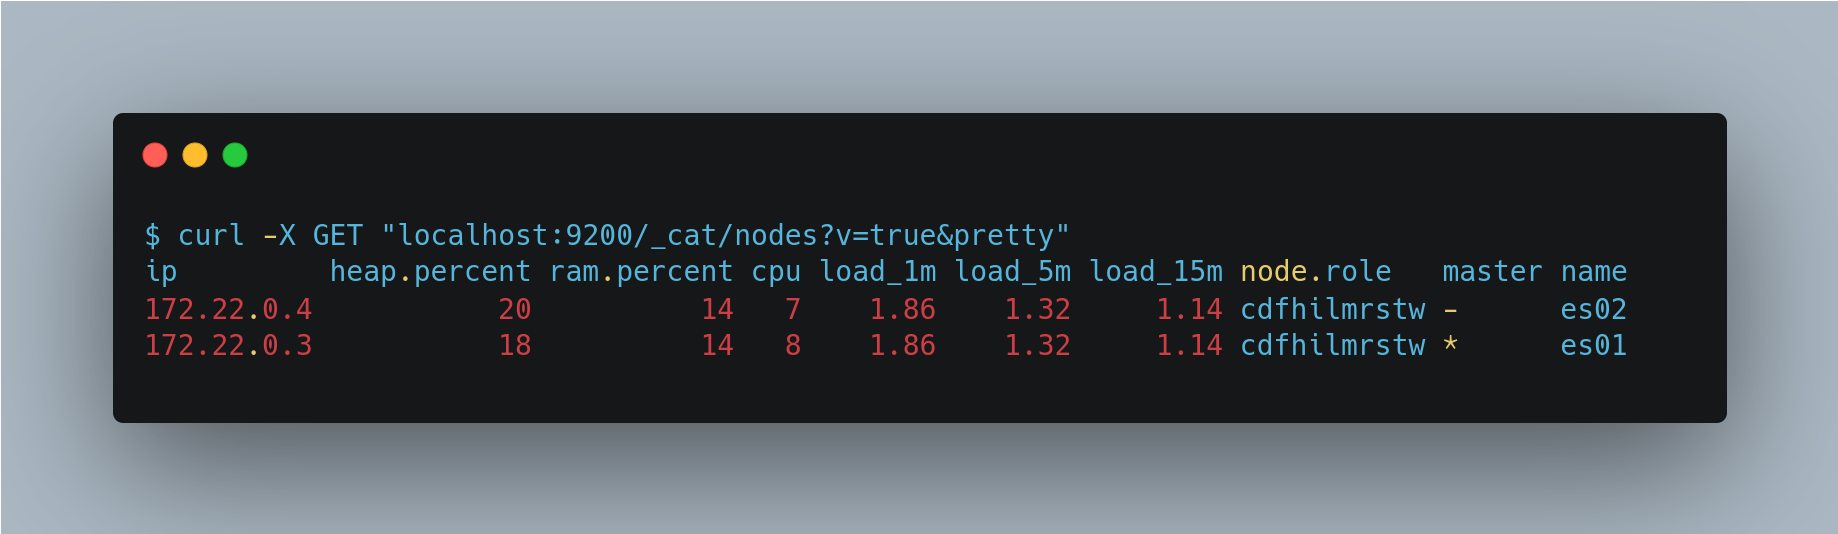
\includegraphics[width=160mm]{curl-different.png}
    \caption{クラスタに参加しているノードを一覧表示した結果}
    \label{p2}
  \end{center}
\end{figure}

図 \ref{p2}より, バージョンが7.17.9である2つのノード(es01, es02)のみが正常にクラスタに参加できていることが確認できる.

また, Elasticsearch起動時に出力されたログを確認したところ, 図 \ref{p3}に示すように, クラスタに参加できなかったes03のコンテナでElasticsearchがエラーログを出力して終了していることが分かった.

\begin{figure}[H]
  \begin{center}
    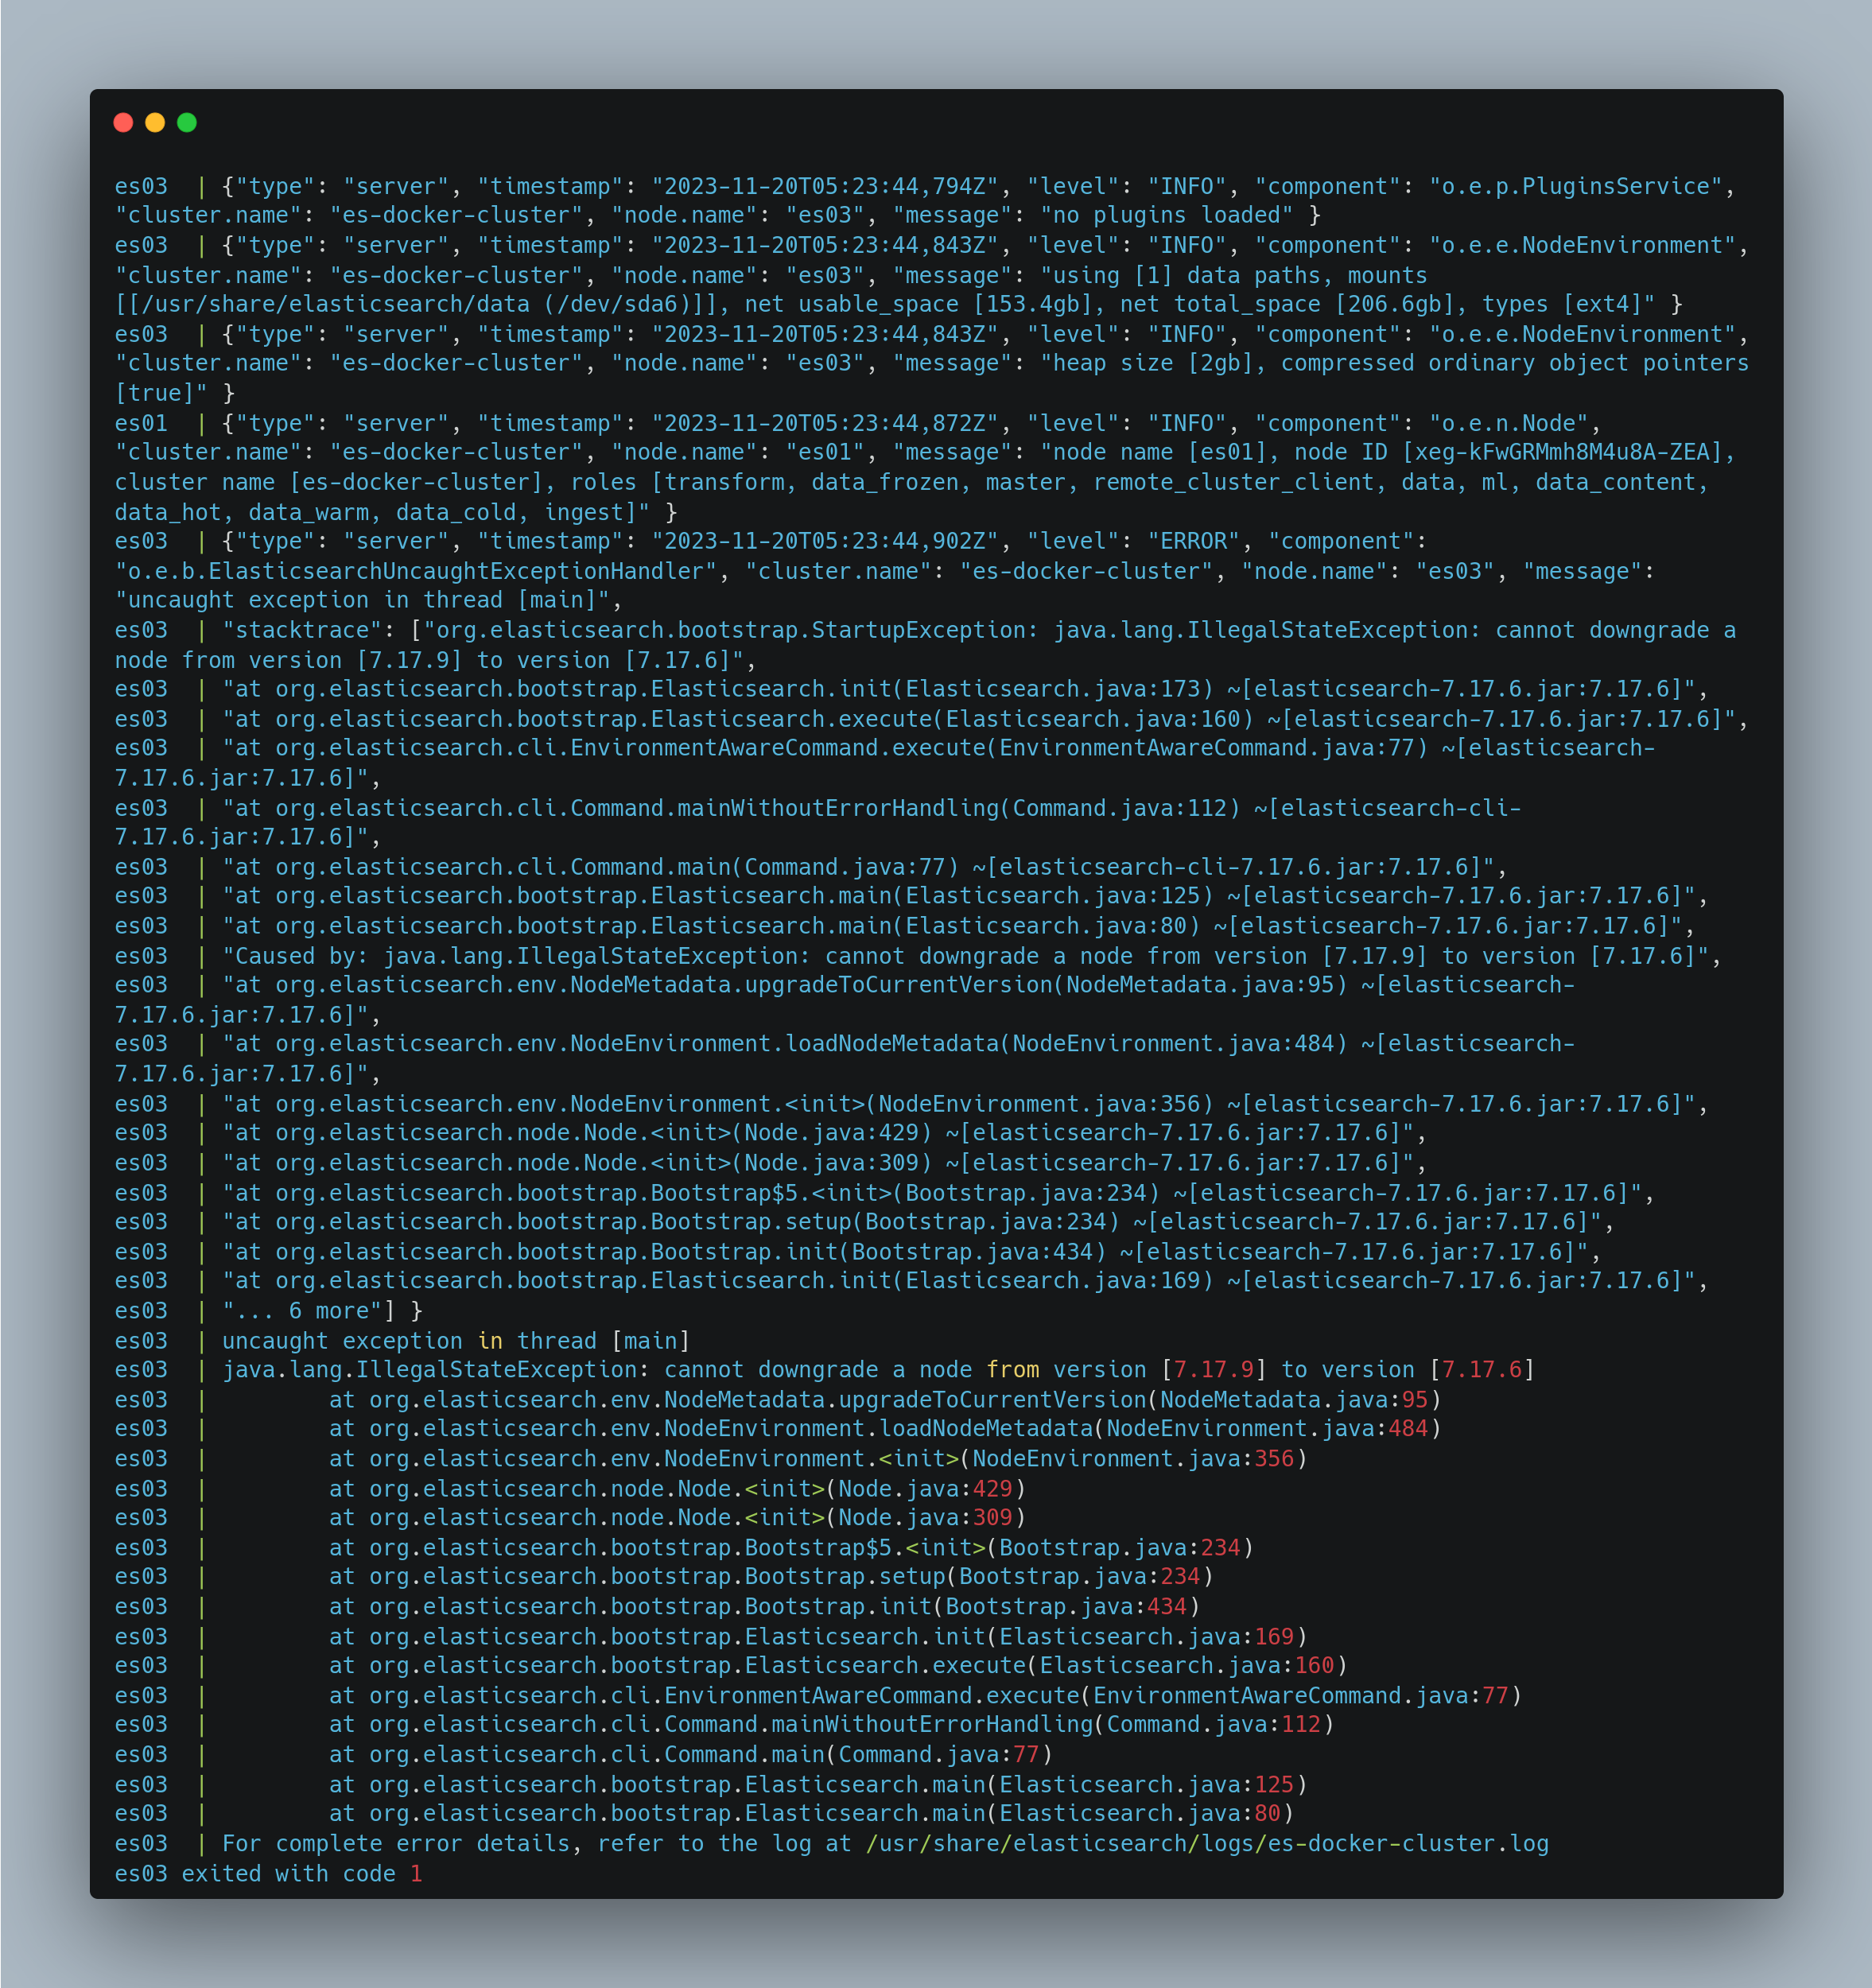
\includegraphics[width=160mm]{log.png}
    \caption{es03のログ}
    \label{p3}
  \end{center}
\end{figure}

\section{まとめ}
今回は, Docker Compose を使用して, 異なるバージョンである7.17.6 と 7.17.9 の Elasticsearch ノードをクラスタリングすることが可能かどうかを確認した.

今回の検証により, 全てのノードが同じ7.17.9バージョンであればクラスタリングを行えることが確認できた. しかし, 異なるマイナーバージョン(今回は7.17.6と7.17.9)のノードでクラスタを構築しようとすると, 古いバージョンのノードはクラスタに参加できなかった.

そのため, リサイクル館の測定データを保存しているElasticsearchをバージョンアップする必要があり, 次回はElasticsearchのバージョンアップ方法について調査した結果を報告する.

\begin{thebibliography}{5}
  \bibitem{1}Elasticsearch B.V.,\\ ”Install Elasticsearch with Docker | Elasticsearch Guide [7.17] | Elastic”, https://www.elastic.co/guide/en/elasticsearch/reference/7.17/docker.html, 参照 Nov 20,2023.
  \bibitem{2}RAKUS Developers Blog, ”Dockerとは一体何なんだ?【初心者向け】 - RAKUS Developers Blog | ラクス エンジニアブログ”, https://tech-blog.rakus.co.jp/entry/20221007/docker, 参照 Nov 20,2023.
\end{thebibliography}

\end{document}

